\chapter{Historia de NeoBilbao}

La historia de NeoBilbao no es una crónica de progreso, sino el registro de una trampa. En menos de un siglo, la colonia pasó de ser una hazaña de solidaridad y supervivencia en un mundo hostil, a convertirse en un matadero industrial y psicológico. Esta es la cronología de cómo el «Acero Azul» y la desesperación de un pueblo se transformaron en su propia condena.

La historia de NeoBilbao arranca en 2052 con la llegada de la flota Euskal-Astra a Ur-Bare, donde los pioneros fundaron una colonia basada en la solidaridad del Auzolan para extraer el codiciado Burdin-Urdin en la Ría de Acero. Sin embargo, la posterior privatización del aire por parte de Orekak-Corp desencadenó la sangrienta Guerra del Plasma (2088--2094), que transformó los Zócalos Industriales en una prisión brutalista. En 2102, tras la implacable Gran Huelga de las Dieciséis Horas, la corporación perpetró la «Cosecha» secuestrando a todos los niños de la colonia para usarlos como procesadores biológicos de ADUR-OS, forzando a los padres a firmar el Etxearen Zina e implantándoles el Velo para anestesiarlos con simulaciones de felicidad mientras entregan sus vidas en la fundición.

\begin{figure}[t]
\centering
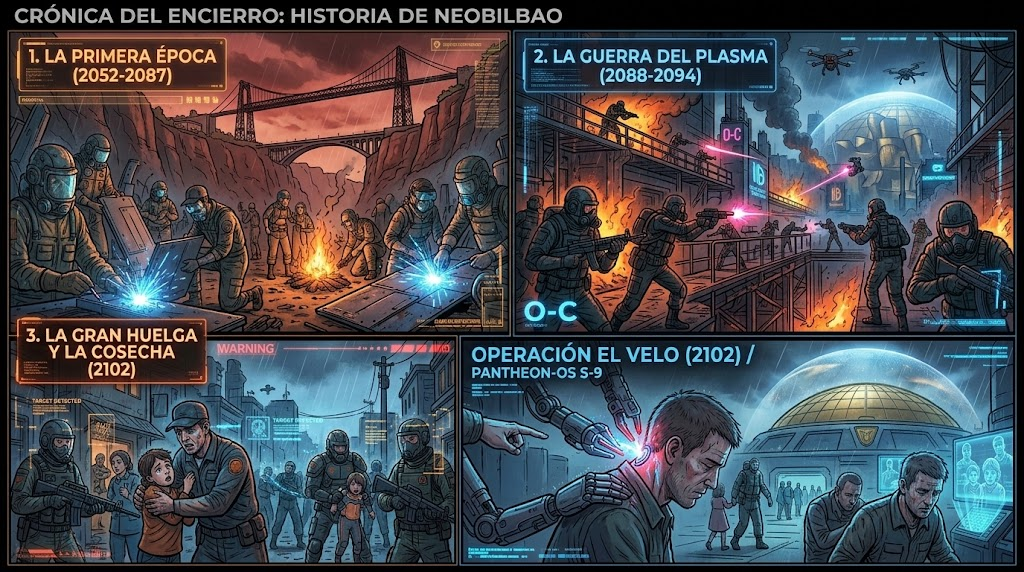
\includegraphics[width=\linewidth]{history.png}
\caption{Crónica del encierro: historia de NeoBilbao.}
\end{figure}

\section{La primera época: el éxodo y la Ría (2052--2087)}

En el año 2052, la expedición de la corporación y consorcio social Euskal-Astra llegó a la órbita del exoplaneta Ur-Bare. Huyendo de una Tierra en colapso, los colonos se encontraron con un mundo desértico, barrido por tormentas de polvo de mineral ferroso y una atmósfera corrosiva. Sin embargo, en las profundidades de la garganta tectónica que hoy llamamos la Ría de Acero, detectaron una anomalía geológica: yacimientos inmensos de Burdin-Urdin (el Acero Azul), un metal superconductor raro capaz de resistir y canalizar energías masivas, vital para el viaje interestelar y la tecnología de soporte de vida.

\lead{La colonización de la garganta.} Los colonos desmontaron las naves de la flota y las encajaron entre las paredes de roca del cañón para crear los primeros asentamientos protegidos, conocidos como los Zócalos. El puente transbordador (inspirado en el puente de Portugalete) fue la primera gran obra de ingeniería, levantado con restos del fuselaje de la nave insignia para conectar los dos lados del abismo y transportar el mineral en bruto.

\lead{El Auzolan industrial.} Durante estas tres primeras décadas, la vida en la colonia se rigió por el Auzolan (el trabajo vecinal y la solidaridad comunitaria). No había salarios ni privilegios; el esfuerzo era colectivo. Si una sección de los Zócalos sufría una filtración de gas, toda la población acudía a sellarla. Las decisiones se tomaban en asambleas abiertas y el reparto de los escasos recursos (agua y aire filtrado) era comunitario. El trabajo en la fundición de Burdin-Urdin era extremadamente duro, pero existía un orgullo compartido: estaban construyendo el hogar para las siguientes generaciones.

\lead{La llegada de la codicia.} Al principio, Orekak-Corp era solo el brazo logístico y tecnológico de la expedición, pero a medida que el valor del Burdin-Urdin se disparaba en los mercados orbitales, la corporación comenzó a monopolizar los suministros de repuestos, los sistemas de filtrado de aire y las patentes de perforación, socavando silenciosamente el gobierno comunal.

\section{La Guerra del Plasma: la privatización del aire (2088--2094)}

Lo que comenzó como una serie de tensiones arancelarias por el control del Burdin-Urdin estalló en un conflicto abierto que cambió para siempre la fisonomía y la sociedad de la colonia. Orekak-Corp decidió que la autogestión de los colonos era ineficiente y que la producción debía multiplicarse por cualquier medio.

\lead{El control del oxígeno.} En 2088, la corporación completó la construcción de la primera fase de la Cúpula Dorada (originalmente un escudo de contención industrial) y, mediante un golpe de fuerza financiero y militar, privatizó el suministro de aire filtrado. De la noche a la mañana, respirar pasó de ser un derecho natural a una deuda acumulable. La corporación introdujo las tarifas de oxígeno y los «créditos de respiración». Aquellos que no podían pagar la cuota eran desplazados a los niveles inferiores, los Zócalos, donde el aire estaba saturado de cenizas y lluvia ácida.

\lead{El choque armado (la Guerra de los Seis Años).} Los trabajadores de la Ría, organizados en milicias vecinales, respondieron con el sabotaje de las refinerías y el bloqueo de las rutas de transporte. La corporación contraatacó militarizando la colonia. Fue un conflicto sucio de guerrillas en los conductos de ventilación y combates a corta distancia entre las naves de carga y las milicias. Orekak-Corp utilizó por primera vez armamento de plasma pesado (que destruyó sectores residenciales enteros de los Zócalos) y desplegó sus primeras unidades de seguridad (Basajaun y Lamiak) para aplastar la resistencia.

\lead{La derrota y el encierro.} En 2094, debilitados por la falta de medicamentos, el hambre y el racionamiento forzado del aire por parte de la corporación, las milicias se rindieron. Orekak-Corp se autoproclamó autoridad única de NeoBilbao, formalizando la división de castas. La Cúpula Dorada se cerró para las élites y la burocracia, mientras que los Zócalos Industriales se convirtieron de facto en prisiones de trabajo de donde ningún obrero (Langile) podía salir sin autorización. La vida comunitaria fue aplastada, sustituida por el control biométrico y la deuda perpetua.

\section{La Gran Huelga y la Cosecha (2102)}

La paz impuesta por las armas era una olla a presión. En 2102, el hacinamiento, la reducción sistemática de las raciones de oxígeno y las jornadas de trabajo insoportables provocaron la mayor rebelión de la historia de la colonia: la Gran Huelga de las Dieciséis Horas.

\lead{El colapso de la colonia.} Los obreros apagaron los altos hornos y ocuparon el puente transbordador y los sistemas de bombeo, bloqueando toda exportación de Burdin-Urdin. Sin la fundición activa, la Cúpula Dorada se quedó sin energía. Durante tres semanas, el Directorio (Batzordea) vio cómo el frío y el desabastecimiento amenazaban con destruir su paraíso. La respuesta militar tradicional no era opción; si destruían los Zócalos, Orekak-Corp perdería la mano de obra y los recursos para siempre. El Directorio necesitaba una sumisión absoluta, definitiva y que no destruyera las fábricas.

\lead{El Proyecto Sugaar y el secuestro generacional.} Ibaizabal-Burdin, bajo las directrices del Batzordea, ejecutó un plan de una crueldad sin precedentes. Utilizando tropas de choque y la División Sorgin, la corporación asaltó los sectores residenciales y de cuidado de los Zócalos, secuestrando en masa a todos los niños de la colonia (la siguiente generación, de entre 2 y 12 años). Fueron trasladados a las profundidades del núcleo, bajo la Cúpula Dorada.

\lead{El chantaje del Etxearen Zina.} Con los niños en su poder, el Directorio emitió un ultimátum a los huelguistas: si no firmaban el Etxearen Zina (el Juramento del Linaje) y volvían al trabajo inmediatamente, sus hijos morirían. El tratado forzaba a los padres a ceder la custodia total de los niños a la corporación, supuestamente para «educarlos y salvarlos del veneno de los Zócalos» en internados de la zona alta. Desesperados y rotos por la amenaza, los Langileak firmaron y volvieron a los hornos.

\lead{La introducción del Velo.} Para garantizar que la rabia no volviera a estallar y que los padres no intentaran asaltar la Cúpula, la corporación instaló obligatoriamente el implante neuronal del Velo (conectado a la red ADUR-OS / Sugaar). En lugar de mantener a la población bajo el terror constante, Orekak-Corp los anestesió con felicidad. El Velo comenzó a proyectar simulaciones y falsas videollamadas de los niños, sanos, sonrientes y agradecidos en un idílico internado superior.

\lead{La verdad oculta.} Los obreros creyeron que sus hijos estaban a salvo, y que su sacrificio valía la pena; el 90\,\% se convirtió voluntariamente en Los Sacrificados. Lo que nadie sospechaba ---y que se convirtió en el secreto más oscuro de la colonia--- es que la corporación no tenía la infraestructura ni el interés de educar a miles de hijos de obreros. En su lugar, los niños fueron conectados a tanques de soporte vital, convirtiendo sus cerebros en el hardware orgánico que mantiene viva la Cúpula. El Velo no era un canal de comunicación; era la pantalla de un matadero digital diseñado para que los padres siguieran picando el mineral que los estaba matando.
